\chapter{Experimentos computacionais}
\label{sec:experimentos}

Neste tópico são apresentados os resultados de experimentos realizados com os algoritmos propostos no tópico \ref{sec:algo}...

\begin{table*}[htbp]
	\centering
	\caption{Pesos utilizados na primeira fase.}
	\label{tab:pesos_primeira_fase}

	\begin{tabular}{|>{\centering}p{2cm}|p{3cm}<{\centering}|}\hline
		\textbf{Peso} & \textbf{Valor} \\ \hline
		$\alpha_{a_3}$ & 1 \\ \hline
		$\alpha_{a_4}$ & 1 \\ \hline
	\end{tabular}
\end{table*}


\section{Planejamento e execução dos experimentos}

Os experimentos foram organizados e executados da seguinte forma:

\begin{description}
	\item[Amostras:] Todas as instâncias ... processos do sistema\footnote{Este procedimento foi seguido para evitar erros ...}.
	
	\item[Tempo de execução:] Na primeira fase ....  
\end{description}


\section{Metodologia de análise dos resultados}
\label{sec:met_analise}

Na análise dos resultados ...
	
	\begin{itemize}
		 \item $pd_{ijk}<1$: significa que ... a instância $i$.
		 
		 \item $pd_{ijk}=1$: significa que a solução $Z_{ijk}$ é uma solução ...	 
	\end{itemize}
	
Quanto a qualidade ...
		
	\begin{enumerate}
		\item \textbf{Distribuição das melhores soluções:} Os algoritmos ...
	
		\item \textbf{Distribuição das soluções médias:} Os algoritmos são ...
	\end{enumerate}			

As melhores soluções ...


%\clearpage
\section{Análise dos Resultados}
\label{sec:results}

 A análise dos resultados ...


%\clearpage
\subsubsection{Distribuição das melhores soluções}

De forma semelhante ...


\clearpage
\subsubsection{Distribuição de todas as soluções}

A \ref{fig:graf_overall_pd_g2} apresenta a distribuição de ...

\begin{figure}[htb]
	\centering
	\subfigure[Grupo 2 - conjunto de todas as soluções representadas em $pd$. \label{fig:graf_overall_pd_g2}]					{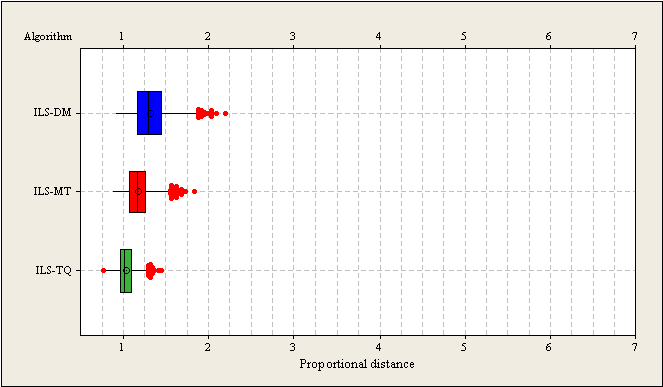
\includegraphics[scale=.51]{graf_overall_pd_g2.png}}
	\subfigure[Grupo 1 - conjunto de todas as soluções representadas em $pd$. \label{fig:graf_overall_pd_g1}]					{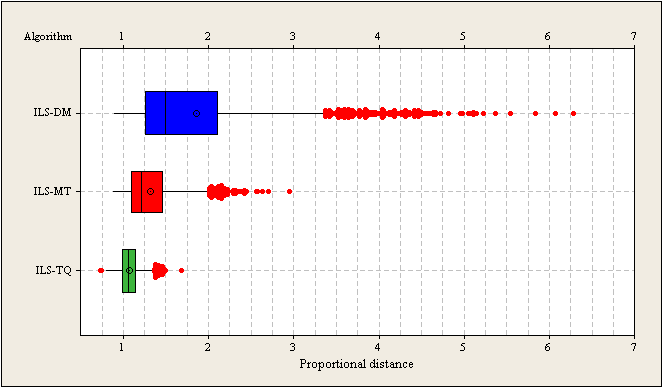
\includegraphics[scale=.51]{graf_overall_pd_g1.png}}	

	\caption{Distribuição de todas as soluções.}
	\label{fig:graf_overall}
\end{figure}

No grupo 2, ...


\clearpage
\subsubsection{Considerações finais}

Como observado nas seções anteriores, quanto ao ...


